\section{Introduction}
\label{sec:intro}

Auditory scene recognition (ASR) \cite{5745009} is the problem of 
classifying an audio sample into one of a set of predefined complex
scenes, each of which may comprise of multiple simple sound events. 
Examples of such scenes include ``street'', ``toilet'', ``restaurant'', 
``park'', etc. A ``toilet'' scene might include simple sound events such as 
urinating, running water, and the hand dryer (see \fig{exa}).
ASR finds many applications in mobile devices, robotics, criminal 
investigation and national security. 
%For example, with ASR, a cell phone
%can detect that it is in a meeting and automatically turn down the volume;
%or plays appropriate music when in different environment to match the activity
%or mood of the user. Another example is crime investigation. Law enforcement
%team can use ASR to recognize the background context of audio recordings from
%wire-tapping, phone conversations, and other sources. In the past, it takes 
%human experts many hours to repeatedly sieve through many audio recordings
%with ad hoc accuracy. ASR automates this process and significantly
%improves the effeciency of crime solving.
%\KZ{This example is weak:
%A sweeping robot can adapt its cleaning mode according to
%it's environments, i.e., streets, classrooms or homes.}
%
%ASR is an interesting problem because i) audio sensors are one of the most
%inexpensive sensors to build and deploy and they are already deployed in
%almost every smart phone; ii) these sensors as well as conventional audio
%recording have created a large amount of digitized audio information and
%much of this is readily available online; iii) the amount of information
%in even high-quality audio information is much smaller than images and videos
%and hence it is easier to store and process; and iv) 
The past century has seen remarkable progress in digital signal processing 
and the Internet era has accumulated large amount of digitized audio 
recordings online, often for free.
%there are many
%mathematical tools for (pre)processing audio signals (either mono or stereo).
Therefore, it appears that we have the necessary ingredients
for solving this important problem. 

\begin{figure}[th]
\centering
\epsfig{file=figures/example.eps,width=\columnwidth}
\caption{A waveform of an audio clip recorded in a toilet}
\label{fig:exa}
\end{figure}
However, ASR still presents a few major challenges. First, even to human beings,
recognizing a scene from an audio clip is not an easy task. Peltonen \et\cite{peltonen2001recognition} remarked that the best humans can do 
for classifying into 25 different scenes is just 70\%. 
Second, even though a number of successful techniques have been developed
for speech recognition, these techniques cannot be directly applied to
auditory scene recognition, despite their similarities, 
because human speech is made up of limited number of phonemes as basic units, 
whereas environmental scenes have much larger variations. 
Thus, understanding and recognizing environmental audio scenes
is a much harder problem.
Third, while it is well known that humans
recognize scenes by detecting simple events 
\cite{peltonen2001recognition,heittola2010audio}, 
it is still difficult to separate the events from a mixture of 
signals or sources 
\cite{comon2010handbook}. Therefore,
most machine learning based approaches do not attempt to recognize the simple
events in an input sample, but instead train models of the scenes directly
from samples. Such approaches have so far met limited success (with best accuracy close to humans \cite{1561288}) because a complex scene can have so many variations
that large number of labeled training samples are required to build 
an accurate model; but such training samples can be hard to obtain.

In this paper, we model the ASR problem as a multi-label classification
problem. Given an audio clip $A$, and a set of terms $S$
that describe different auditory scenes, such as ``street'', ``toilet'',
``train station'', etc. The output of the problem is a classification
label $l \in S$ which best characterizes the context or scene
under which $A$ was recorded. 
we adopt a big-data, knowledge driven approach in which
we derive knowledge about the relationships between a scene and its
constituent events from large text corpus and comprehensive concept and
word taxonomies. This allows us to build {\em scene-event} mappings 
for virtually any environmental scenes without supervised training.
Then separately, we can train auditory detection models for each
primitive events such as car honks and dog barks, from audio clips from
the web. With these primitive models, we will then be able to detect
the probability distributions of events in an input audio sample, and 
thus infer the likelihood of a particular scene according to the
scene-event map. For this paper, we focus our attention on mono audio samples,
but techniques developed here can be readily adapted to stereo sounds.

%Recently, mobile devices become more and more important in people's life. At the same time, some location/context based tools and apps are developed, which are very useful. For example, a mobile phone can automatically turn itself into silent mode while in a meeting. A portable audio player can play appropriate musics in different scenes. Thus, scene recognition attracts more and more attention.
%
%The audio effects, such as {\em phone-ringing}, {\em car-horn}, etc., play a important role in our daily life. Comparing with other data, such as image data and video data, audio data is much more easier to get. For example, mobile phone can capture audio information from all around, all directions. Besides, audio data can record a lot of information related to scene/activity/context.
%
%Therefore, audio data can be used to infer/recognize/classify current scene/activity/context. Although this work is similar to speech recognition, there are lots of differences. For example, speech has the limited size of phonemes as natural basic units, while environmental sound does not have them. Thus, understanding environmental sound and infer the scene is still an open problem.
%
%In early listening test conducted in \cite{peltonen2001recognition}, human beings are able to recognize daily scenes in $70\%$ accuracy on average, and confusions come among those contexts that shares some same prominent audio events. Therefore, we can conclude that for human beings, the audio events are the most important part to recognize audio context.
%
%Some previous work \cite{1621215, heittola2010audio} used the audio events to do scene recognition. All of their work obtained a good accuracy. However, they chose the audio events and labeled them manually, and might not have good expansion.
%
%In this paper, we will propose an event-based audio scenes recognition system using knowledge bases. Our approach assumes that different audio scenes can be distinguished by some audio events. 

The main contributions of our work are:
\begin{itemize}
\item This paper is first-of-its-kind research which combines text mining with
audio event detection into an unsupervised auditory scene recognition 
framework that requires no human intervention. The approach can be used to
handle scenes for which very few audio samples are available 
(\secref{sec:approach}).
\item We leverage a large number of online movie and TV scripts to 
train probabilistic models of common scenes based on audible concepts.
This approach can scale up to very complex and unusual scenes. While
we showcase this technique using movie and drama scripts, more scenes
can be modeled from other textual corpuses such as novels, personal stories,
news and even the general web pages 
(\secref{sec:vocab} and \secref{sec:mapping}).
%We use knowledge base and text data to build the probabilistic model of audio events and scenes rather than using audio data directly. Thus our model can be more precise, since it is much easier to find a huge number of text data than audio data. Also, text processing is much faster than audio processing.
%\item Our system can download and label training data automatically, instead of doing manual work. All of our training data are download directly from Internet without manual pre-precessing. Therefore, our system is more scalable than previous work.
%\item We propose a method to cluster audio event training data where 
%each cluster represents a particular type of that event, e.g., a certain
%species of dog for the ``dog'' event, or a certain aspect of an event.
%The clustering approach effectively removes noises in the training data
%and improves the quality of the models for the primitive events 
%(\secref{sec:audiotrain}).
\item Our ASR framework achieves average accuracy of 42\% for
a 10-scene classification task. 
This is on par with the best performing method from 2013 AASP Challenge 
using training data of the scenes themselves (\secref{sec:eval}). 
%After clustering, 
%we use different model to describe different cluster, which can reduce the impact of low quality data.
\end{itemize}

%Our system is designed as \fig{sys}. We will introduce each part in next sections.

